\documentclass[10pt,a4paper]{article}

\usepackage[utf8]{inputenc}
\usepackage[T1]{fontenc}

%%%%%%%%%%% Own packages
\usepackage[a4paper, margin=1in]{geometry}
\usepackage{multicol}
\usepackage{lipsum}

% Header/footer
\usepackage{fancyhdr}
\pagestyle{fancy}
\renewcommand{\headrulewidth}{0pt}


% Maths
%\usepackage{physics}
\usepackage{esdiff}
\usepackage{cancel}
\usepackage{amstext,amsbsy,amssymb,mathtools}
\usepackage{times} 
\usepackage{siunitx}
\usepackage{tensor}

%% Graphics
\usepackage{caption}
\captionsetup{margin=20pt,font=small,labelfont=bf}
%\renewcommand{\thesubfigure}{(\alph{subfigure})} % Style: 1(a), 1(b)
%\pagestyle{empty}
\usepackage{graphicx} % Include figure files

% Listsings and items
\usepackage[page]{appendix}
\usepackage[shortlabels]{enumitem}
\setenumerate{wide,labelwidth=!, labelindent=0pt}
\usepackage{varioref}
\usepackage{hyperref}
\usepackage{cleveref}

% Paragraph indent and skip
\setlength{\parindent}{2em}
\setlength{\parskip}{1em}
\setlength\extrarowheight{5pt}

%% User units
\DeclareSIUnit \parsec {pc}

%% User commands
\providecommand{\qwhere}
{
    \ensuremath{
    ,\quad \text{where} \quad 
    }
}

\title{AST5220 Cosmology \rm{II}\\ 
\vspace{5mm}Milestone 1 - The Background Cosmology}
\author{Jakob Borg}
%%%%%%%
\begin{document}
%%%%%%%

\maketitle

\lhead{Milestone 1 AST5220}
\rhead{Jakobbor}
%%%%%%%%

\section{Brief Introduction}
\label{sec:Intro}
In this first milestone\footnote{First of four milestones.} our goal is to solve for the evolution of the uniform background cosmology of our universe. With a set of cosmological parameters the numerical code developed here will use the Friedmann equation to produce the Hubble parameter and solve for the conformal time, both as functions of some time variable from the early Universe to today and beyond.

\section{Theory}
\label{sec:Theory}
\subsection{The Friedmann Equation}
\label{subsec:Theory/Friedmann}
Assuming a homogeneous and isotropic Universe, where each energy component act as a perfect fluid, we can derive the Friedmann equation from Einstein's theory of general relativity. Expressed in terms of density we write the equation as
%
\begin{equation}
    H^2 = \frac{8\pi G}{3} \sum_i \rho_i \qwhere H = \frac{1}{a}\diff{a}{t} = \frac{\dot{a}}{a}
    \label{eq:Friedmann_density}
\end{equation}
%
and the sum goes over each component contributing to the energy density of the Universe. In our case we consider the components baryons ($B$), cold dark matter ($CDM$), radiation ($R$), the cosmological constant ($\lambda$), curvature ($K$) and neutrinos ($\nu$). By using the critical density $\rho_c$, which is the density required for a perfectly flat universe, we introduce the relative density parameters $\Omega_i$ for each component
%
\begin{equation}
    \Omega_i = \frac{\rho_i}{\rho_c} \qwhere \rho_c = \frac{3H^2}{8\pi G}.
    \label{eq:Omega_i}
\end{equation}
%
In our close to perfectly flat universe we then have that the sum of the density parameters should equal unity
%
\begin{equation}
    \sum_i \Omega_i = 1.
    \label{eq:Omega_sum}
\end{equation}
%
To simplify the calculations we assume no contribution from the curvature, $\Omega_K=0$, and we neglect the tiny contribution from the neutrinos, $\Omega_\nu = 0$. Most of the today's value of these relative density parameters we can measure, and the last one may be obtained through the others using \cref{eq:Omega_sum}. In the end we want to express \cref{eq:Friedmann_density} in terms of these known parameters.

\subsection{Energy and Matter Densities}
\label{subsec:Theory/densities}
By conservation of mass and energy we also have the continuity equation for each component
%
\begin{equation}
    \dot{\rho_i} + 3H \left(\rho_i + P_i \right) = 0.
    \label{eq:continuity equation}
\end{equation}
%
Here we define the equation of state on the form $\omega = \frac{P}{\rho}$ and solve \cref{eq:continuity equation} for the density in terms of $\omega$ and the scale factor $a$. The solutions will be on the form
%
\begin{equation}
    \rho_i = \rho_{i,0} a^{-3(1+\omega_i)}
    \label{eq:rho_i(a,w)}
\end{equation}
%
where subscripts $0$ indicate today's values and the equation of state parameter for each component is known. The densities are presented in \cref{tab:densities} together with expressions for the relative density parameters.
%
\begin{table}[h]
    \centering
    \begin{tabular}{|l|c|l|l|}
    \hline
    Component & $\omega$      & \multicolumn{1}{c|}{$\rho(a)$} & \multicolumn{1}{c|}{$\Omega(a)$}        \\[3pt] \hline
    $CDM$     & $0$           & $\rho_{CDM,0}a^{-3}$           & $\frac{H_0^2}{H^2}\Omega_{CDM,0}a^{-3}$ \\[3pt] \hline
    $B$       & $0$           & $\rho_{B,0}a^{-3}$             & $\frac{H_0^2}{H^2}\Omega_{B,0}a^{-3}$   \\[3pt] \hline
    $R$       & $\frac{1}{3}$ & $\rho_{R,0}a^{-4}$             & $\frac{H_0^2}{H^2}\Omega_{R,0}a^{-4}$   \\[3pt] \hline
    $\Lambda$ & $-1$          & $\rho_{\Lambda,0}$             & $\frac{H_0^2}{H^2}\Omega_{\Lambda,0}$   \\[3pt] \hline
    \end{tabular}
    \caption{Table of density and relative density expressions as functions of scale factor $a$ and present day values (subscript $0$) for each component. The expressions for the relative density parameters derived in \cref{asec:density_params}.}
    \label{tab:densities}
\end{table}
%
\subsection{Conformal Time}
\label{subsce:Theory/Conformal Time}
The last quantity we want, which will be the main focus of the computation in this milestone, is the conformal time. This is the maximum distance that light may have traveled since the big bang, which will be dependent on the expansion of the Universe. Here we used the differential form of the conformal time, defined as 
%
\begin{equation}
    \diff{\eta}{t} = \frac{c}{a}.
    \label{eq:eta_diff}
\end{equation}
%

\section{Method}
\label{sec:Method}
\subsection{Time Variable}
\label{subsec:Method/Time variable}
The default choice of the scale factor as time variable is used in the equations listed in \cref{sec:Theory}. In order to get the required time resolution in the rapidly evolving early universe all the way to today we instead use the logarithmic scale factor, $x= \ln(a)$, as our main time variable in all the calculations. The results will be presented in terms of this logarithmic time variable, as well as the redshift $z$ defined as
%
\begin{equation}
    1+z = \frac{1}{a} = \frac{1}{\exp(x)}.
    \label{eq:redshift}
\end{equation}

\subsection{Code Implementation}
\label{subsec:Method/Code Implementation}

\subsubsection{Cosmological Parameters}
\label{subsubsec:Method/Cosmological parameters}
The known cosmological parameters given as input to our code and are listed in \cref{tab:input_parameters}. These are used as a basis for all our calculations.
%
\begin{table}[h]
    \centering
    \begin{tabular}{|l|l|}
    \hline
    Parameter      & Value    \\ \hline
    $h$            & $0.7$    \\ \hline
    $T_{CMB}$      & $2.7255$ \\ \hline
    $\Omega_{B,0}$     & $0.046$  \\ \hline
    $\Omega_{CDM,0}$ & $0.224$  \\ \hline
    \end{tabular}
    \caption{Cosmological parameters given as input to our code. Values taken from observations. Listed are the unitless Hubble constant $h$, the mean temperature of cosmic microwave background $T_{CMB}$ and the present day relative densities for baryons and cold dark matter.}
    \label{tab:input_parameters}
\end{table}
%

With this input we first find the Hubble parameter today and the remaining nonzero density parameters\footnote{The methods and calculations for the densities of neutrinos and curvature is still in the code to keep it general, for possible further expansion of the project to include these terms. As they stand they only return zero and will not affect the calculations.}
%
\begin{alignat}{2}
    H_0 &= 100h\,\si{\km\per\s\per\mega\parsec} &&= \SI{2.26855e-18}{s}\label{eq:H0}
    \\
    \Omega_R &= \frac{2\pi^2}{30}\frac{\left(k_bT_{CMB}\right)^4}{\hbar^3c^5}\frac{8\pi G}{3H_0^2} &&= \num{5.04688e-5} \label{eq:OmegaR0}
    \\
    \Omega_\Lambda &= 1 - \sum_{i\neq \Lambda} \Omega_i &&= \num{0.72995} \label{eq:OmegaLambda0}.
\end{alignat}
%
\subsection{Get Methods}
\label{subsec:Method/Get methods}
Using the preferred time variable, the expressions listed for the relative density parameters in \cref{tab:densities} are rewritten into functions of $x$ and implemented as separate methods.

The expressions for the densities in \cref{eq:Friedmann_density} are rewritten using the critical density, the present day values of the relative density parameters and their time dependence 
%
\begin{equation}
    \rho_i = \rho_{c,0} \Omega_{i,0} a^{-3(1+\omega_i)} = \frac{3H_0^2}{8\pi G}\Omega_{i,0} a^{-3(1+\omega_i)}.
\end{equation}
%
The final form of the Friedmann equation implemented as its own method in the code then reads
%
\begin{equation}
    H = H_0 \sqrt{\left(\Omega_{B,0}+\Omega_{CDM,0}\right)\exp(-3x) + \Omega_{R,0}\exp(-4x) + \Omega_{\Lambda,0}}.
    \label{eq:Friedmann implemented} 
\end{equation}

We also define the "Hubble prime" parameter
%
\begin{equation}
    \mathcal{H} = aH.
    \label{eq:Hprime}
\end{equation}
This is essentially the same as $\dot{a}$, and can be thought of as the rate of the expansion of the Universe. This quantity, together with its first and second derivative, will be used more in the milestones to come. For now we can use them to benchmark the implementation of our code, see \cref{asec:Benchmarking} for the expressions and the results of the testing. $\mathcal{H}$ is also used in the expression for the conformal time, which is the final part of our implementation.

\subsection{Solving the Conformal Time}
\label{subsec:Method/Conformal time}
By the chain rule we can rewrite \cref{eq:eta_diff} first into a differential equation in $a$, and then into $x$, as follows
\begin{alignat}{2}
    \diff{\eta}{t} &= \diff{\eta }{a}\diff{a}{t} = \diff{\eta }{a}\mathcal{H} = \frac{c}{a} & \qquad \Rightarrow \diff{\eta }{a} &= \frac{c}{a\mathcal{H}} \notag
    \\
    \diff{\eta }{x} &= \diff{\eta }{a}\diff{a}{x} \qwhere \diff{a}{x} = a & \qquad \Rightarrow \diff{\eta }{x} &= \frac{c}{\mathcal{H}(x).} \label{eq:eta_diff_of_x}
\end{alignat}
With this simple ordinary differential equation (ODE) we used the provided ODEsolver, wrapping GSL's Runge-Kutta 4 algorithm, to solve the system. As we are using the logarithmic scale factor we have some trouble defining our initial condition numerically, which should be $\eta(a=0)=0$. We cannot start our time variable $x$ at $a=0$, which corresponds to $x\to-\infty$, so instead we first used a wide range of x-values, $x\in[-25,3]$, to solve the system with an approximation for the initial condition $\eta(x=-25)=0$. Then we compute a spline of the result, and use this spline to evaluate the solution in a more well behaved range of values, $x\in[-15,2]$. Finally all the results are evaluated in this smaller range of $x$-values using the implemented methods and plotted using "Python".

\section{Results}
\label{sec:Results}
First we present the evolution of the relative energy densities of the Universe, shown in \cref{fig:omegas_of_x}. Here each component is plotted, together with the combined contribution from all matter ($CDM + B$.) We see three distinct regimes where each component is dominating, radiation domination marked with blue, matter domination marked with red and lastly the present day regime dominated by the cosmological constant marked in green. This color coding is used to better visualize these regimes in all the produced plots.

\begin{figure}[ht]
    \centering
    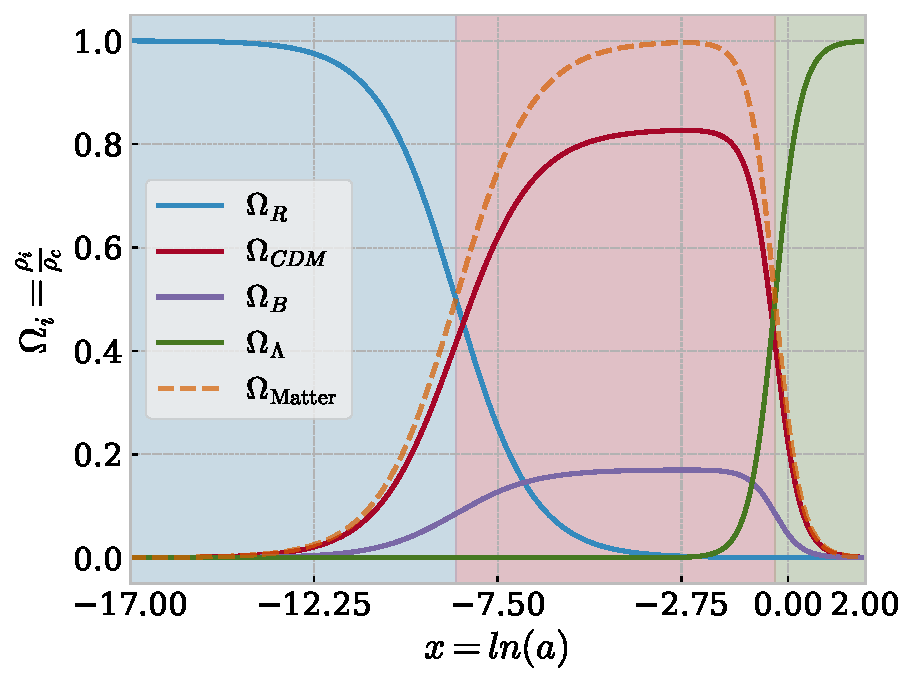
\includegraphics[scale=0.5]{../figs/omegas_of_x.pdf}
    \caption{}
    \label{fig:omegas_of_x}
\end{figure}

\begin{figure}[ht]
    \centering
    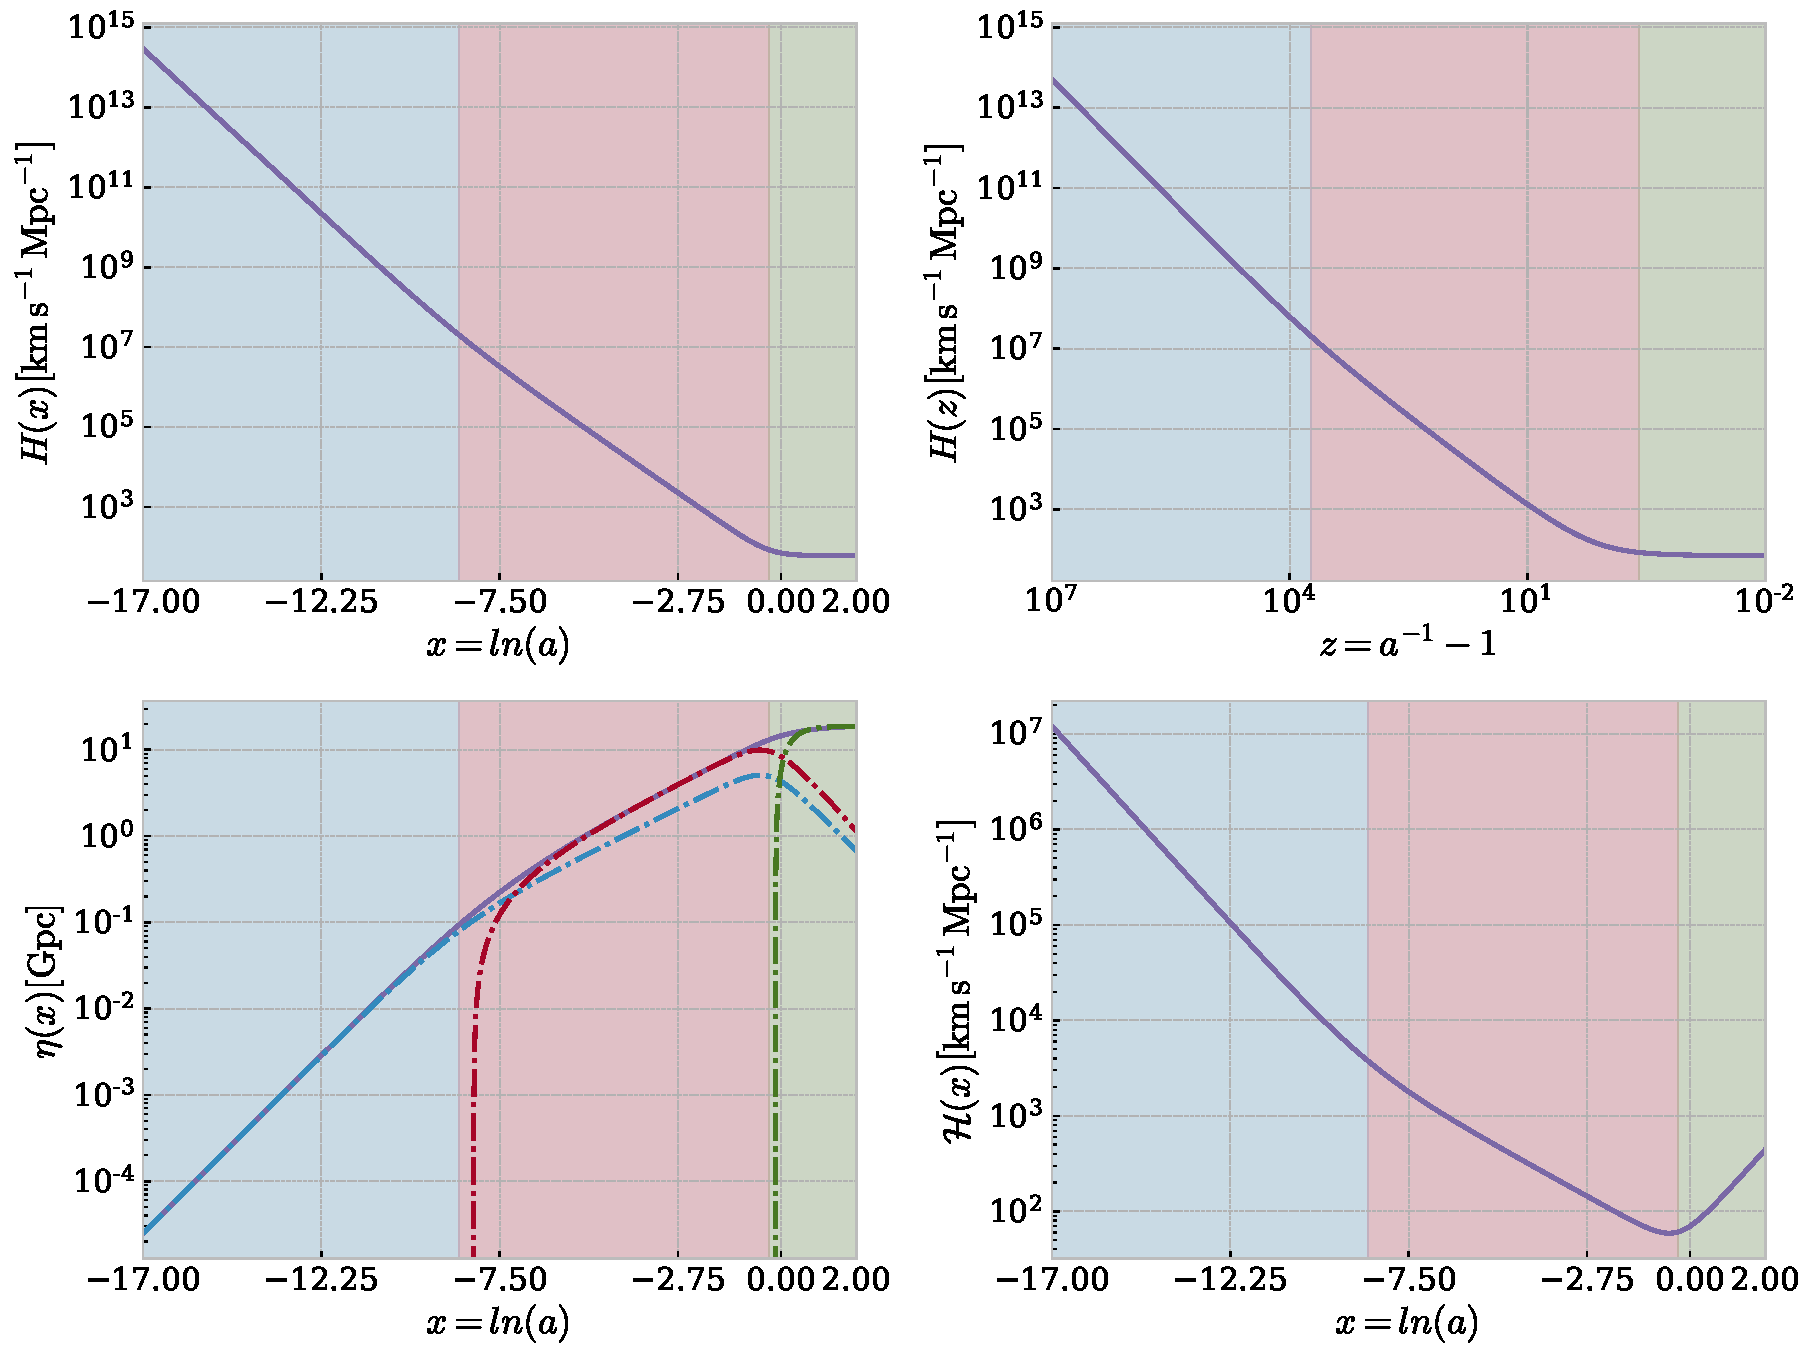
\includegraphics[scale=0.5]{../figs/Hubble_eta_of_x.pdf}
    \caption{Testcaption3}
    \label{fig:hubbe_and_eta}
\end{figure}

\newpage
\begin{appendices}
\appendix
\section{Expressions for the relative density parameters}
\label{asec:density_params}
The expressions for the relative density parameters presented in \cref{tab:densities} is obtained in the following way.
\begin{align*}
    \Omega_i & = \frac{\rho_i}{\rho_c} = \frac{1}{\rho_c} \rho_{i,0} a^{-3(1+\omega_i)} \quad \bigg\rvert \cdot \rho_{c,0} = \frac{3H_0^2}{8\pi G}
    \\
    & = \frac{\rho_{c,0}}{\rho_c} \frac{\rho_{i,0}}{\rho_{c,0}} a^{-3(1+\omega_i)} \qwhere \frac{\rho_{i,0}}{\rho_{c,0}} = \Omega_{i,0} \quad \text{and} \quad \frac{\rho_{c,0}}{\rho_c} = \frac{H_0^2}{H^2}
    \\
    \Rightarrow \Omega_i (a) & = \frac{H_0^2}{H^2} \Omega_{i,0} a^{-3(1+\omega_i)} 
\end{align*}

\section{Benchmarking the Code}
\label{asec:Benchmarking}


\end{appendices}

\end{document}